\documentclass[../tc_tpfinal_main.tex]{subfiles}

\begin{document}

%capítulo
\chapter{Filtro}

\section{Introducción}

\section{Análisis de sensibilidades}
\subsection{Celda Sallen-Key Pasabandas}
\begin{center}
$w_0 = \sqrt{\frac{\frac{\mathrm{R_1}}{\mathrm{R_3}} + 1}{\mathrm{C_1}\, \mathrm{C_2}\, \mathrm{R_1}\, \mathrm{R_2}}}
;$
$Q = \frac{\sqrt{\frac{\mathrm{R_1}}{\mathrm{R_3}} + 1}}{\sqrt{\frac{\mathrm{C_1}\, \mathrm{R_1}}{\mathrm{C_2}\, \mathrm{R_2}}} - \left(\frac{\mathrm{R_1}\, \mathrm{r_b}}{\mathrm{R_3}\, \mathrm{r_a}} - 1\right)\, \sqrt{\frac{\mathrm{C_2}\, \mathrm{R_2}}{\mathrm{C_1}\, \mathrm{R_1}}} + 1}
;$
$G = \frac{\frac{\mathrm{r_b}}{\mathrm{r_a}} + 1}{\frac{\mathrm{R_1}\, \left(\frac{\mathrm{C_1}}{\mathrm{C_2}} + 1\right)}{\mathrm{R_2}} - \frac{\mathrm{R_1}\, \mathrm{r_b}}{\mathrm{R_3}\, \mathrm{r_a}} + 1}
;$
\end{center}

Obtenemos analíticamente las expresiones de las sensibilidades relativas de Q para algunos componentes: \par

$S^{G}_{R_1} = -\frac{\mathrm{R_1}\, \left(\frac{\frac{\mathrm{C_1}}{\mathrm{C_2}} + 1}{\mathrm{R_2}} - \frac{\mathrm{r_b}}{\mathrm{R_3}\, \mathrm{r_a}}\right)}{\frac{\mathrm{R_1}\, \left(\frac{\mathrm{C_1}}{\mathrm{C_2}} + 1\right)}{\mathrm{R_2}} - \frac{\mathrm{R_1}\, \mathrm{r_b}}{\mathrm{R_3}\, \mathrm{r_a}} + 1}$\par

$S^{G}_{R_2} = \frac{\mathrm{R_1}\, \left(\frac{\mathrm{C_1}}{\mathrm{C_2}} + 1\right)}{\mathrm{R_2}\, \left(\frac{\mathrm{R_1}\, \left(\frac{\mathrm{C_1}}{\mathrm{C_2}} + 1\right)}{\mathrm{R_2}} - \frac{\mathrm{R_1}\, \mathrm{r_b}}{\mathrm{R_3}\, \mathrm{r_a}} + 1\right)}$\par

$S^{G}_{R_3} = -\frac{\mathrm{R_1}\, \mathrm{r_b}}{\mathrm{R_3}\, \mathrm{r_a}\, \left(\frac{\mathrm{R_1}\, \left(\frac{\mathrm{C_1}}{\mathrm{C_2}} + 1\right)}{\mathrm{R_2}} - \frac{\mathrm{R_1}\, \mathrm{r_b}}{\mathrm{R_3}\, \mathrm{r_a}} + 1\right)}$\par

$S^{G}_{R_4} = 0$\par

$S^{G}_{r_a} = -\frac{\mathrm{r_a}\, \mathrm{r_b}\, \left(\mathrm{C_1}\, \mathrm{R_1}\, \mathrm{R_3} + \mathrm{C_2}\, \mathrm{R_1}\, \mathrm{R_2} + \mathrm{C_2}\, \mathrm{R_1}\, \mathrm{R_3} + \mathrm{C_2}\, \mathrm{R_2}\, \mathrm{R_3}\right)}{\left(\mathrm{r_a} + \mathrm{r_b}\right)\, \left(\mathrm{C_1}\, \mathrm{R_1}\, \mathrm{R_3}\, \mathrm{r_a} + \mathrm{C_2}\, \mathrm{R_1}\, \mathrm{R_3}\, \mathrm{r_a} + \mathrm{C_2}\, \mathrm{R_2}\, \mathrm{R_3}\, \mathrm{r_a} - \mathrm{C_2}\, \mathrm{R_1}\, \mathrm{R_2}\, \mathrm{r_b}\right)}$\par

$S^{G}_{r_b} = \frac{\mathrm{r_a}\, \mathrm{r_b}\, \left(\mathrm{C_1}\, \mathrm{R_1}\, \mathrm{R_3} + \mathrm{C_2}\, \mathrm{R_1}\, \mathrm{R_2} + \mathrm{C_2}\, \mathrm{R_1}\, \mathrm{R_3} + \mathrm{C_2}\, \mathrm{R_2}\, \mathrm{R_3}\right)}{\left(\mathrm{r_a} + \mathrm{r_b}\right)\, \left(\mathrm{C_1}\, \mathrm{R_1}\, \mathrm{R_3}\, \mathrm{r_a} + \mathrm{C_2}\, \mathrm{R_1}\, \mathrm{R_3}\, \mathrm{r_a} + \mathrm{C_2}\, \mathrm{R_2}\, \mathrm{R_3}\, \mathrm{r_a} - \mathrm{C_2}\, \mathrm{R_1}\, \mathrm{R_2}\, \mathrm{r_b}\right)}$\par

$S^{G}_{C_1} = -\frac{\mathrm{C_1}\, \mathrm{R_1}}{\mathrm{C_2}\, \mathrm{R_2}\, \left(\frac{\mathrm{R_1}\, \left(\frac{\mathrm{C_1}}{\mathrm{C_2}} + 1\right)}{\mathrm{R_2}} - \frac{\mathrm{R_1}\, \mathrm{r_b}}{\mathrm{R_3}\, \mathrm{r_a}} + 1\right)}$\par

$S^{G}_{C_2} = \frac{\mathrm{C_1}\, \mathrm{R_1}}{\mathrm{C_2}\, \mathrm{R_2}\, \left(\frac{\mathrm{R_1}\, \left(\frac{\mathrm{C_1}}{\mathrm{C_2}} + 1\right)}{\mathrm{R_2}} - \frac{\mathrm{R_1}\, \mathrm{r_b}}{\mathrm{R_3}\, \mathrm{r_a}} + 1\right)}$\par

$S^{w_0}_{R_1} = -\frac{\mathrm{R_3}}{2\, \left(\mathrm{R_1} + \mathrm{R_3}\right)}$\par

$S^{w_0}_{R_2} = - \frac{1}{2}$\par
$S^{w_0}_{R_3} = -\frac{\mathrm{R_1}}{2\, \left(\mathrm{R_1} + \mathrm{R_3}\right)}$\par

$S^{w_0}_{R_4} = 0$\par

$S^{w_0}_{r_a} = 0$\par

$S^{w_0}_{r_b} = 0$\par

$S^{w_0}_{C_1} = - \frac{1}{2}$\par

$S^{w_0}_{C_2} = - \frac{1}{2}$\par

$S^{Q}_{R_1} = -\frac{\mathrm{r1}\, \left(\frac{\sqrt{\frac{\mathrm{r1}}{\mathrm{r3}} + 1}\, \left(\frac{\mathrm{c1}}{2\, \mathrm{c2}\, \mathrm{r2}\, \sqrt{\frac{\mathrm{c1}\, \mathrm{r1}}{\mathrm{c2}\, \mathrm{r2}}}} - \frac{\mathrm{rb}\, \sqrt{\frac{\mathrm{c2}\, \mathrm{r2}}{\mathrm{c1}\, \mathrm{r1}}}}{\mathrm{r3}\, \mathrm{ra}} + \frac{\mathrm{c2}\, \mathrm{r2}\, \left(\frac{\mathrm{r1}\, \mathrm{rb}}{\mathrm{r3}\, \mathrm{ra}} - 1\right)}{2\, \mathrm{c1}\, {\mathrm{r1}}^2\, \sqrt{\frac{\mathrm{c2}\, \mathrm{r2}}{\mathrm{c1}\, \mathrm{r1}}}}\right)}{{\left(\sqrt{\frac{\mathrm{c1}\, \mathrm{r1}}{\mathrm{c2}\, \mathrm{r2}}} - \left(\frac{\mathrm{r1}\, \mathrm{rb}}{\mathrm{r3}\, \mathrm{ra}} - 1\right)\, \sqrt{\frac{\mathrm{c2}\, \mathrm{r2}}{\mathrm{c1}\, \mathrm{r1}}} + 1\right)}^2} - \frac{1}{2\, \mathrm{r3}\, \sqrt{\frac{\mathrm{r1}}{\mathrm{r3}} + 1}\, \left(\sqrt{\frac{\mathrm{c1}\, \mathrm{r1}}{\mathrm{c2}\, \mathrm{r2}}} - \left(\frac{\mathrm{r1}\, \mathrm{rb}}{\mathrm{r3}\, \mathrm{ra}} - 1\right)\, \sqrt{\frac{\mathrm{c2}\, \mathrm{r2}}{\mathrm{c1}\, \mathrm{r1}}} + 1\right)}\right)\, \left(\sqrt{\frac{\mathrm{c1}\, \mathrm{r1}}{\mathrm{c2}\, \mathrm{r2}}} - \left(\frac{\mathrm{r1}\, \mathrm{rb}}{\mathrm{r3}\, \mathrm{ra}} - 1\right)\, \sqrt{\frac{\mathrm{c2}\, \mathrm{r2}}{\mathrm{c1}\, \mathrm{r1}}} + 1\right)}{\sqrt{\frac{\mathrm{r1}}{\mathrm{r3}} + 1}}$\par

$S^{Q}_{R_2} = \frac{\mathrm{R_2}\, \left(\frac{\mathrm{C_2}\, \left(\frac{\mathrm{R_1}\, \mathrm{r_b}}{\mathrm{R_3}\, \mathrm{r_a}} - 1\right)}{2\, \mathrm{C_1}\, \mathrm{R_1}\, \sqrt{\frac{\mathrm{C_2}\, \mathrm{R_2}}{\mathrm{C_1}\, \mathrm{R_1}}}} + \frac{\mathrm{C_1}\, \mathrm{R_1}}{2\, \mathrm{C_2}\, {\mathrm{R_2}}^2\, \sqrt{\frac{\mathrm{C_1}\, \mathrm{R_1}}{\mathrm{C_2}\, \mathrm{R_2}}}}\right)}{\sqrt{\frac{\mathrm{C_1}\, \mathrm{R_1}}{\mathrm{C_2}\, \mathrm{R_2}}} - \left(\frac{\mathrm{R_1}\, \mathrm{r_b}}{\mathrm{R_3}\, \mathrm{r_a}} - 1\right)\, \sqrt{\frac{\mathrm{C_2}\, \mathrm{R_2}}{\mathrm{C_1}\, \mathrm{R_1}}} + 1}$\par

$S^{Q}_{R_3} = -\frac{\mathrm{R_1}\, \left(\mathrm{R_3}\, \mathrm{r_a} + \mathrm{R_3}\, \mathrm{r_a}\, \sqrt{\frac{\mathrm{C_1}\, \mathrm{R_1}}{\mathrm{C_2}\, \mathrm{R_2}}} + \mathrm{R_3}\, \mathrm{r_a}\, \sqrt{\frac{\mathrm{C_2}\, \mathrm{R_2}}{\mathrm{C_1}\, \mathrm{R_1}}} + \mathrm{R_1}\, \mathrm{r_b}\, \sqrt{\frac{\mathrm{C_2}\, \mathrm{R_2}}{\mathrm{C_1}\, \mathrm{R_1}}} + 2\, \mathrm{R_3}\, \mathrm{r_b}\, \sqrt{\frac{\mathrm{C_2}\, \mathrm{R_2}}{\mathrm{C_1}\, \mathrm{R_1}}}\right)}{2\, \left(\mathrm{R_1} + \mathrm{R_3}\right)\, \left(\mathrm{R_3}\, \mathrm{r_a} + \mathrm{R_3}\, \mathrm{r_a}\, \sqrt{\frac{\mathrm{C_1}\, \mathrm{R_1}}{\mathrm{C_2}\, \mathrm{R_2}}} + \mathrm{R_3}\, \mathrm{r_a}\, \sqrt{\frac{\mathrm{C_2}\, \mathrm{R_2}}{\mathrm{C_1}\, \mathrm{R_1}}} - \mathrm{R_1}\, \mathrm{r_b}\, \sqrt{\frac{\mathrm{C_2}\, \mathrm{R_2}}{\mathrm{C_1}\, \mathrm{R_1}}}\right)}$\par

$S^{Q}_{R_4} = 0$\par

$S^{Q}_{r_a} = -\frac{\mathrm{R_1}\, \mathrm{r_b}\, \sqrt{\frac{\mathrm{C_2}\, \mathrm{R_2}}{\mathrm{C_1}\, \mathrm{R_1}}}}{\mathrm{R_3}\, \mathrm{r_a}\, \left(\sqrt{\frac{\mathrm{C_1}\, \mathrm{R_1}}{\mathrm{C_2}\, \mathrm{R_2}}} - \left(\frac{\mathrm{R_1}\, \mathrm{r_b}}{\mathrm{R_3}\, \mathrm{r_a}} - 1\right)\, \sqrt{\frac{\mathrm{C_2}\, \mathrm{R_2}}{\mathrm{C_1}\, \mathrm{R_1}}} + 1\right)}$\par

$S^{Q}_{r_b} = \frac{\mathrm{R_1}\, \mathrm{r_b}\, \sqrt{\frac{\mathrm{C_2}\, \mathrm{R_2}}{\mathrm{C_1}\, \mathrm{R_1}}}}{\mathrm{R_3}\, \mathrm{r_a}\, \left(\sqrt{\frac{\mathrm{C_1}\, \mathrm{R_1}}{\mathrm{C_2}\, \mathrm{R_2}}} - \left(\frac{\mathrm{R_1}\, \mathrm{r_b}}{\mathrm{R_3}\, \mathrm{r_a}} - 1\right)\, \sqrt{\frac{\mathrm{C_2}\, \mathrm{R_2}}{\mathrm{C_1}\, \mathrm{R_1}}} + 1\right)}$\par

$S^{Q}_{C_1} = -\frac{\mathrm{C_1}\, \left(\frac{\mathrm{R_1}}{2\, \mathrm{C_2}\, \mathrm{R_2}\, \sqrt{\frac{\mathrm{C_1}\, \mathrm{R_1}}{\mathrm{C_2}\, \mathrm{R_2}}}} + \frac{\mathrm{C_2}\, \mathrm{R_2}\, \left(\frac{\mathrm{R_1}\, \mathrm{r_b}}{\mathrm{R_3}\, \mathrm{r_a}} - 1\right)}{2\, {\mathrm{C_1}}^2\, \mathrm{R_1}\, \sqrt{\frac{\mathrm{C_2}\, \mathrm{R_2}}{\mathrm{C_1}\, \mathrm{R_1}}}}\right)}{\sqrt{\frac{\mathrm{C_1}\, \mathrm{R_1}}{\mathrm{C_2}\, \mathrm{R_2}}} - \left(\frac{\mathrm{R_1}\, \mathrm{r_b}}{\mathrm{R_3}\, \mathrm{r_a}} - 1\right)\, \sqrt{\frac{\mathrm{C_2}\, \mathrm{R_2}}{\mathrm{C_1}\, \mathrm{R_1}}} + 1}$\par

$S^{Q}_{C_2} = \frac{\mathrm{C_2}\, \left(\frac{\mathrm{R_2}\, \left(\frac{\mathrm{R_1}\, \mathrm{r_b}}{\mathrm{R_3}\, \mathrm{r_a}} - 1\right)}{2\, \mathrm{C_1}\, \mathrm{R_1}\, \sqrt{\frac{\mathrm{C_2}\, \mathrm{R_2}}{\mathrm{C_1}\, \mathrm{R_1}}}} + \frac{\mathrm{C_1}\, \mathrm{R_1}}{2\, {\mathrm{C_2}}^2\, \mathrm{R_2}\, \sqrt{\frac{\mathrm{C_1}\, \mathrm{R_1}}{\mathrm{C_2}\, \mathrm{R_2}}}}\right)}{\sqrt{\frac{\mathrm{C_1}\, \mathrm{R_1}}{\mathrm{C_2}\, \mathrm{R_2}}} - \left(\frac{\mathrm{R_1}\, \mathrm{r_b}}{\mathrm{R_3}\, \mathrm{r_a}} - 1\right)\, \sqrt{\frac{\mathrm{C_2}\, \mathrm{R_2}}{\mathrm{C_1}\, \mathrm{R_1}}} + 1}$\par

Reemplazando las expresiones anteriores por los valores teóricos de los componentes, obtenemos:
			 	\begin{table}[H] 
				\centering
 				\begin{tabular}{||c c c c c c c c||} 
 					\hline
				  Parámetro& $R_1$ & $R_2$ & $R_3$ & $r_a$ & $r_b$&$C_1$&$C_2$\\ [0.5ex] 
 					\hline\hline
					 $S^G_x$& -0.2788& 1.4425& -1.1637&-1.7811&1.7811&-0.7212&0.7212\\
					 $S^{w_0}_x$& $-0.25$ &$-0.5$&-0.25&$0$&$0$&$-0.5$&$-0.5$\\
					 $S^{Q}_x$ &$0.8319$& 0.5819& -1.4137&$-1.1637$&$1.1637$&$-0.5819$&$0.5819$\\[1ex] 
					\hline
				\end{tabular}
			\end{table}
\subsection{Celda Sallen-Key Pasa-altos}
\begin{figure}[H]	
	\centering
	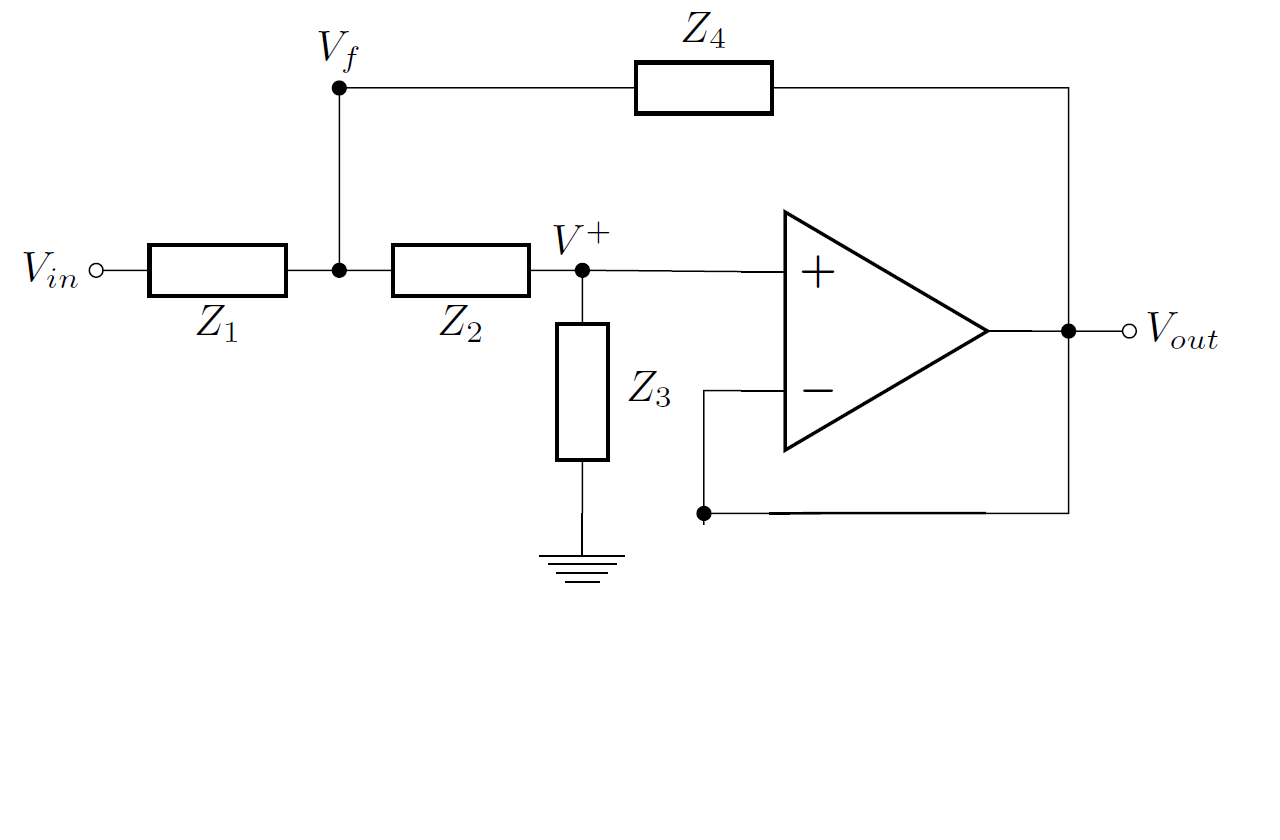
\includegraphics[scale=0.5]{imagenes/sallen_key_circ.png}
	\caption{Celda Sallen-Key Pasa-altos}
	\label{fig:tpfinal_sallen_key_circ}
\end{figure}

Obtenemos analíticamente las expresiones de las sensibilidades relativas de Q para algunos componentes: \par
$S^{Q}_{C_1} =-\frac{\mathrm{C_1} - \mathrm{C_2}}{2\, \left(\mathrm{C_1} + \mathrm{C_2}\right)}$ \par
$S^{Q}_{C_2} = \frac{\mathrm{C_1} - \mathrm{C_2}}{2\, \left(\mathrm{C_1} + \mathrm{C_2}\right)}$ \par 
El resto de las sensibilidades derivan directamente valores numéricos, por lo que reemplazando las expresiones anteriores por los valores teóricos de los componentes, obtenemos:\par
 	\begin{table}[H] 
				\centering
 				\begin{tabular}{||c c c c c||} 
 					\hline
				  Parámetro& $R_1$ & $R_2$&$C_1$&$C_2$\\ [0.5ex] 
 					\hline\hline
					 $S^{w_0}_x$& $- \frac{1}{2}$ &$- \frac{1}{2}$&$- \frac{1}{2}$&$- \frac{1}{2}$\\
					 $S^{Q}_x$&$- \frac{1}{2}$ &$\frac{1}{2}$&0&0\\[1ex] 
					\hline
				\end{tabular}
			\end{table}
\subsection{Celda Sallen-Key Pasa-altos con factor ganancia}
\begin{figure}[H]	
	\centering
	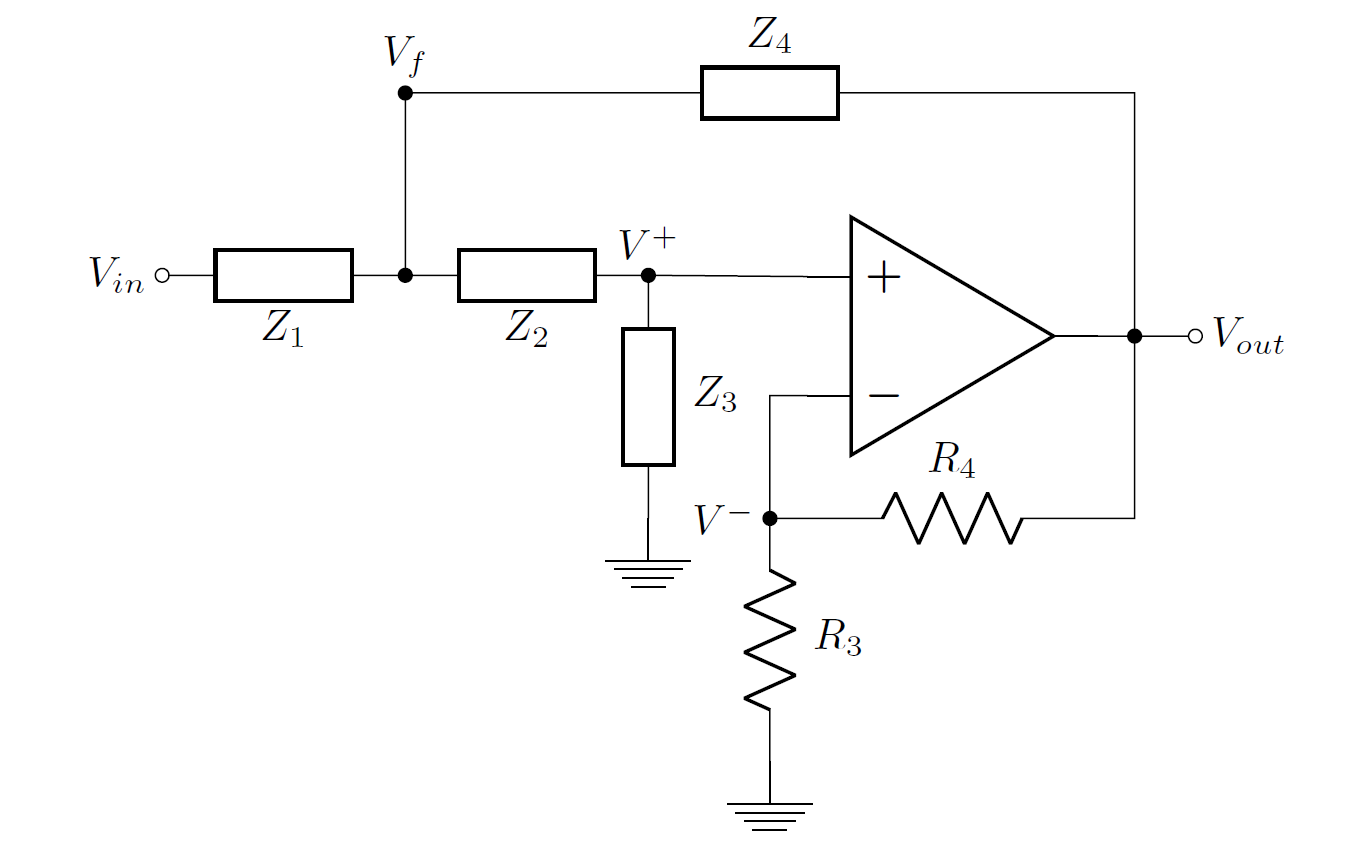
\includegraphics[scale=0.5]{imagenes/sallen_key_gain_circ.png}
	\caption{Celda Sallen-Key Pasa-altos con factor ganancia}
	\label{fig:tpfinal_sallen_key_gain_circ}
\end{figure}

Obtenemos analíticamente las expresiones de las sensibilidades relativas para Q y para G para algunos componentes: \par

$S^{Q}_{R_1} = -\frac{\mathrm{C_1}\, \mathrm{R_1}\, \mathrm{R_3} + \mathrm{C_2}\, \mathrm{R_1}\, \mathrm{R_3} + \mathrm{C_2}\, \mathrm{R_2}\, \mathrm{R_4}}{2\, \mathrm{C_1}\, \mathrm{R_1}\, \mathrm{R_3} + 2\, \mathrm{C_2}\, \mathrm{R_1}\, \mathrm{R_3} - 2\, \mathrm{C_2}\, \mathrm{R_2}\, \mathrm{R_4}}
$ \par
$S^{Q}_{R_2} = \frac{\mathrm{C_1}\, \mathrm{R_1}\, \mathrm{R_3} + \mathrm{C_2}\, \mathrm{R_1}\, \mathrm{R_3} + \mathrm{C_2}\, \mathrm{R_2}\, \mathrm{R_4}}{2\, \mathrm{C_1}\, \mathrm{R_1}\, \mathrm{R_3} + 2\, \mathrm{C_2}\, \mathrm{R_1}\, \mathrm{R_3} - 2\, \mathrm{C_2}\, \mathrm{R_2}\, \mathrm{R_4}}
$\par
$S^{Q}_{R_3} = -\frac{\mathrm{C_2}\, \mathrm{R_2}\, \mathrm{R_4}}{\mathrm{R_3}\, \left(\mathrm{R_1}\, \left(\mathrm{C_1} + \mathrm{C_2}\right) - \frac{\mathrm{C_2}\, \mathrm{R_2}\, \mathrm{R_4}}{\mathrm{R_3}}\right)}
$\par
$S^{Q}_{R_4} = \frac{\mathrm{C_2}\, \mathrm{R_2}\, \mathrm{R_4}}{\mathrm{R_3}\, \left(\mathrm{R_1}\, \left(\mathrm{C_1} + \mathrm{C_2}\right) - \frac{\mathrm{C_2}\, \mathrm{R_2}\, \mathrm{R_4}}{\mathrm{R_3}}\right)}
$\par
$S^{Q}_{C_1} = -\frac{\mathrm{C_1}\, \mathrm{R_1}\, \mathrm{R_3} - \mathrm{C_2}\, \mathrm{R_1}\, \mathrm{R_3} + \mathrm{C_2}\, \mathrm{R_2}\, \mathrm{R_4}}{2\, \mathrm{C_1}\, \mathrm{R_1}\, \mathrm{R_3} + 2\, \mathrm{C_2}\, \mathrm{R_1}\, \mathrm{R_3} - 2\, \mathrm{C_2}\, \mathrm{R_2}\, \mathrm{R_4}}
$\par
$S^{Q}_{C_2} = \frac{\mathrm{C_1}\, \mathrm{R_1}\, \mathrm{R_3} - \mathrm{C_2}\, \mathrm{R_1}\, \mathrm{R_3} + \mathrm{C_2}\, \mathrm{R_2}\, \mathrm{R_4}}{2\, \mathrm{C_1}\, \mathrm{R_1}\, \mathrm{R_3} + 2\, \mathrm{C_2}\, \mathrm{R_1}\, \mathrm{R_3} - 2\, \mathrm{C_2}\, \mathrm{R_2}\, \mathrm{R_4}}
$ \par

$S^G_{R_3} = -\frac{\mathrm{R_4}}{\mathrm{R_3} + \mathrm{R_4}}$\par
$S^G_{R_4} = \frac{\mathrm{R_4}}{\mathrm{R_3} + \mathrm{R_4}}$\par

El resto de las sensibilidades derivan directamente valores numéricos, por lo que reemplazando las expresiones anteriores por los valores teóricos de los componentes, obtenemos:\par

			 	\begin{table}[H] %datos thd simulado
				\centering
 				\begin{tabular}{||c c c c c c c||} 
 					\hline
				  Parámetro& $R_1$ & $R_2$ & $R_3$ & $R_4$&$C_1$&$C_2$\\ [0.5ex] 
 					\hline\hline
					 $S^G_x$& 0& 0&-0.4842&0.4842&0&0\\
					 $S^{w_0}_x$& -0.5 &-0.5& 0& 0&-0.5&-0.5\\
					  $S^{Q}_x$& -1.8931 &1.8931&-1.3931& 1.3931&-0.7535&0.7535\\[1ex] 
					\hline
				\end{tabular}
			\end{table}
\subsection{Celda Tow-Thomas}

\begin{figure}[H]	
	\centering
	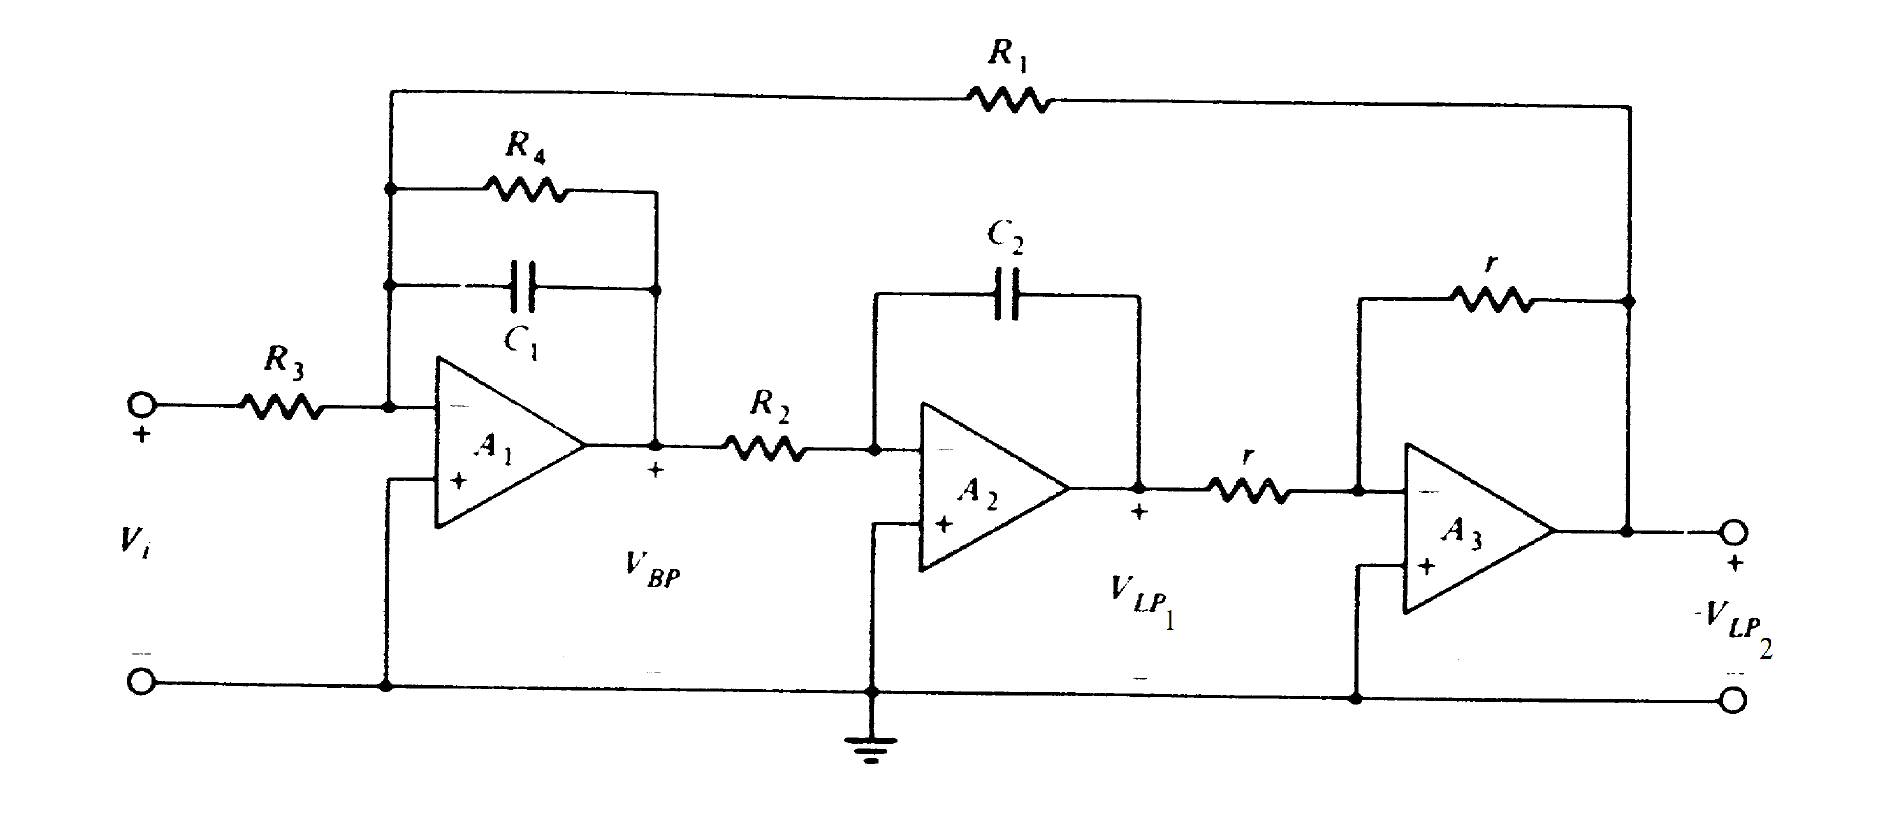
\includegraphics[scale=0.5]{imagenes/tow_thomas_circ.png}
	\caption{Celda Tow-Thomas}
	\label{fig:tpfinal_tow_thomas_circ}
\end{figure}

Se despeja la transferencia total del sistema:\par
\begin{center}
$H(s) = -\frac{\mathrm{R_1}\, \mathrm{R_4}\, \mathrm{r_b}}{\mathrm{R_3}\, \left(\mathrm{C_1}\, \mathrm{C_2}\, \mathrm{R_1}\, \mathrm{R_2}\, \mathrm{R_4}\, \mathrm{r_b}\, s^2 + \mathrm{C_2}\, \mathrm{R_1}\, \mathrm{R_2}\, \mathrm{r_a}\, s + \mathrm{R_4}\, \mathrm{r_b}\right)}
$
\end{center}

De la cual se despejan los siguientes parámetros:\par

\begin{center}
$w_0 = \sqrt{\frac{r_b}{C_1\cdot C_2\cdot R_1\cdot R_2\cdot r_a}}; $
%wo = sqrt(r_b/(C_1*C_2*R_1*R_2*r_a))
$Q = \sqrt{\frac{C_1\cdot r_b}{C_2\cdot R_1\cdot R_2\cdot r_a}}; $
%Q = R_4*sqrt(C_1*r_b/(C_2*R_1*R_2*r_a));
$G = -\frac{R_1}{R_4}; $ 
\end{center}

para la ganancia, obtenemos las sensibilidades con respecto a todos los componentes:\par

 	\begin{table}[H] %datos thd simulado
				\centering
 				\begin{tabular}{||c c c c c c c c c||} 
 					\hline
				  Parámetro& $R_1$ & $R_2$ & $R_3$ & $R_4$ & $r_a$ & $r_b$&$C_1$&$C_2$\\ [0.5ex] 
 					\hline\hline
					 $S^G_x$& 1 & 0& -1& 0&0&0&0&0\\
					 $S^{w_0}_x$& $- \frac{1}{2}$ &$- \frac{1}{2}$& 0& 0&$- \frac{1}{2}$&$- \frac{1}{2}$&$- \frac{1}{2}$&$- \frac{1}{2}$\\
					 $S^{Q}_x$&$- \frac{1}{2}$ &$- \frac{1}{2}$& 0& 1&$- \frac{1}{2}$&$- \frac{1}{2}$&$- \frac{1}{2}$&$- \frac{1}{2}$\\[1ex] 
					\hline
				\end{tabular}
			\end{table}
		
\end{document}